\documentclass[11pt, A4paper,norsk]{article}
\usepackage[utf8]{inputenc}
\usepackage[T1]{fontenc}
\usepackage{babel}
\usepackage{amsmath}
\usepackage{amsfonts}
\usepackage{amsthm}
\usepackage{amssymb}
\usepackage[colorlinks]{hyperref}
\usepackage{listings}
\usepackage{color}
\usepackage{hyperref}
\usepackage{graphicx}
\usepackage{cite}
\usepackage{textcomp}
\usepackage{float}

\definecolor{dkgreen}{rgb}{0,0.6,0}
\definecolor{gray}{rgb}{0.5,0.5,0.5}
\definecolor{daynineyellow}{rgb}{1.0,0.655,0.102}
\definecolor{url}{rgb}{0.1,0.1,0.4}

\lstset{frame=tb,
	language=Python,
	aboveskip=3mm,
	belowskip=3mm,
	showstringspaces=false,
	columns=flexible,
	basicstyle={\small\ttfamily},
	numbers=none,
	numberstyle=\tiny\color{gray},
	keywordstyle=\color{blue},
	commentstyle=\color{daynineyellow},
	stringstyle=\color{dkgreen},
	breaklines=true,
	breakatwhitespace=true,
	tabsize=3
}

\lstset{inputpath="C:/Users/Torstein/Documents/UiO/Fys2140/Python programmer"}
\graphicspath{{C:/Users/Torstein/Documents/UiO/Fys2140/"Python programmer"/}}
\hypersetup{colorlinks, urlcolor=url}

\author{Torstein Solheim Ølberg}
\title{Svar på Oblig nr. 8 i Fys2140}



%\lstinputlisting{Filnavn! type kodefil}
%\includegraphics[width=12.6cm,height=8cm]{Filnavn! type png}



\begin{document}
\maketitle
	\begin{center}
\Large \textbf{Oppgaver}
	\end{center}









		\paragraph{1.}
			\subparagraph{a)}
				\begin{flushleft}
TUSL for posisjonene $x \leq 0$ blir
$$\frac{d^2 \psi}{dx^2} = - \frac{2 m E}{\hbar^2} \psi = - k^2 \psi$$
der $k = \frac{\sqrt{2 m E}}{\hbar}$. Vi velger at energien $E$ er positiv fordi ellers får vi en bunden tilstand. Da er den generelle løsningen
$$\psi(x) = A e^{i k x} + B e^{- i k x}$$
TUSL for $x > 0$ blir
$$\frac{d^2 \psi}{dx^2} = - \frac{2 m}{\hbar^2} (E - V_0) \psi = \iota^2 \psi$$
der $\iota = \frac{\sqrt{- 2 m (E - V_0)}}{\hbar}$. $V_0$ er her en positiv konstant som er større enn $E$ og derfor er $\iota$ også positiv og reell. Den generelle løsningen vi får nå må derfor være $e^{i\iota x}$ siden vi ikke har noen partikler fra høyre(antar vi). Så vi får
$$\psi(x) = C e^{\iota x}$$
Nå kan vi finne $\frac{d \psi}{dx}$ for de to forskjellige $\psi$ene.
$$\frac{d \psi}{dx} = ikAe^{ikx} - ikBe^{-ikx} \vee \iota Ce^{\iota x}$$
Til slutt putter vi dette sammen ved hjelp av betingelsen at $\psi(x)$ og $\frac{d \psi}{dx}$ alltid er kontinuerlige, altså at de er like i punktet $x = 0$. Da ender vi opp med
				\end{flushleft}
				\begin{gather*}
A + B = C \\
I : A = C - B \\
II : B = C - A \\
III : ikA - ikB = \iota C \\
\text{Setter $I$ inn i $III$} \\
ik(C - B) - ikB = \iota C \\
ikC - ikB - ikB = \iota C \\
ikC - \iota C = ikB + ikB \\
C (ik - \iota) = 2 i k B \\
B = \frac{C (ik - \iota)}{2 i k} \\
\text{Setter $II$ inn i $III$} \\
ikA - ik(C - A) = \iota C \\
2 i k A = C (ik + \iota) \\
A = \frac{C (ik + \iota)}{2 i k}
				\end{gather*}
				\begin{flushleft}
Finner så $R$ ved realasjonen $R = \frac{|B|^2}{|A|^2}$
				\end{flushleft}
				\begin{gather*}
R = \left( \frac{\frac{C(ik - \iota)}{2ik}}{\frac{C(ik + \iota)}{2ik}} \right)^2 = \frac{(ik - \iota)^2}{(ik + \iota)^2} = \frac{( i \frac{\sqrt{2 m E}}{\hbar} - \frac{\sqrt{2 m(E - V_0)}}{\hbar})^2}{(i \frac{\sqrt{2 m E}}{\hbar} + \frac{\sqrt{2 m(E - V_0)}}{\hbar})^2} = \frac{(i \sqrt{E} - \sqrt{E - V_0})^2}{(i \sqrt{E} + \sqrt{E - V_0})^2} \\
\frac{(i \sqrt{E} - \sqrt{E - V_0})^2}{(i \sqrt{E} + \sqrt{E - V_0})^2} = \frac{(i\sqrt{E} - \sqrt{E - V_0})^2(- i\sqrt{E} + \sqrt{E - V_0})^2}{(E - V_0)^2 + 2 E (E - V_0) + E^2} \\
R = \frac{(i\sqrt{E} - \sqrt{E - V_0})^4}{E^2 - 2 E V_0 + V_0^2 + 2 E^2 - 2 E V_0 + E^2} = \frac{(\sqrt{E} - \sqrt{V_0 - E})^4}{4E^2 - 4 E V_0 + V_0^2} \\
R\left( \frac{V_0}{2} \right) = \lim_{E \rightarrow \frac{V_0}{2}} \frac{(\sqrt{E} - \sqrt{V_0 - E})^4}{4E^2 - 4 E V_0 + V_0^2} = \frac{4(\frac{1}{2} \frac{1}{\sqrt{E}} + \frac{1}{2} \frac{1}{\sqrt{V_0 - E}})^3}{8E - 4V_0} = \frac{(- \frac{1}{2} \frac{1}{\sqrt{E}^3} - \frac{1}{2} \frac{1}{\sqrt{V_0 - E}^3})^2}{8} \\
R\left( \frac{V_0}{2} \right) = \frac{1}{4 V_0^3}
				\end{gather*}
				\begin{flushleft}
Ser at det alltid vil være noe refleksjon med mindre potensialet blir $0$, noe som gir mening, men at jo mindre energien er, jo mer blir reflektert. Samtidig ser vi også at når energien nærmer seg potensialet, går $R$ fortsatt mot $1$. Til slutt ser vi også at $R$ ikke er definert hvis energien er halvparten så stor som potensialet, $\frac{1}{V_0^3}$ når energien nærmer seg $\frac{V_0}{2}$.
				\end{flushleft}









			\subparagraph{b)}
				\begin{flushleft}
Løsningen av TUSL for $x \leq 0$ er samme som tidligere
$$\psi(x) = Ae^{i k x} + Be^{- i k x}$$
TUSL for $x > 0$ blir
$$\frac{d^2 \psi}{dx^2} = - \frac{2 m}{\hbar^2} (E - V_0) = - \iota^2 \psi$$
der $\iota = \frac{\sqrt{2 m (E - V_0)}}{\hbar}$ som blir en positiv, reell konstant siden $E$ alltid er større enn $V_0$. Så da får vi løsningen
$$\psi(x) = C e^{i \iota x}$$
siden vi kan anta at det ikke kommer noe stråling fra høyre. Så regner vi ut den deriverte for begge $\psi$ene
$$\frac{d \psi}{dx} = i k A e^{i k x} - i k B e^{- i k x} \vee i \iota C e^{i \iota x}$$
Setter alt sammen i punktet $x = 0$ sånn som tidligere.
				\end{flushleft}
				\begin{gather*}
I : A = C - B \wedge II : C - A \\
III : ikA - ikB = i \iota C
\text{Setter $I$ inn i $III$} \\
k(C - 2B) = \iota C \\
C(k - \iota) = 2 k B \Rightarrow B = \frac{C(k - \iota)}{2 k} \\
\text{Setter $II$ inn i $III$} \\
k(2A - C) = \iota C \\
C(k + \iota) = 2 k A \Rightarrow A = \frac{C(k + \iota)}{2 k} \\
				\end{gather*}
				\begin{flushleft}
Så finner jeg $R$ på samme måte som over.
				\end{flushleft}
				\begin{gather*}
R = \frac{|B|^2}{|A|^2} = \frac{\left( \frac{C(k - \iota)}{2 k} \right)^2}{\left( \frac{C(k + \iota)}{2 k} \right)^2} = \frac{\left( k - \iota \right)^2}{\left( k + \iota \right)^2} = \frac{\left( \frac{\sqrt{2 m E}}{\hbar} - \frac{\sqrt{2 m (E - V_0)}}{\hbar} \right)^2}{\left( \frac{\sqrt{2 m E}}{\hbar} + \frac{\sqrt{2 m (E - V_0)}}{\hbar} \right)^2} = \frac{\left( \sqrt{E} - \sqrt{E - V_0} \right)^2}{\left( \sqrt{E} + \sqrt{E - V_0} \right)^2} \\
\frac{\left( \sqrt{E} - \sqrt{E - V_0} \right)^4}{E^2 - 2 E (E - V_0) + (E - V_0)^2} = \frac{\left( \sqrt{E} - \sqrt{E - V_0} \right)^4}{E^2 - 2 E^2 + 2 E V_0 + E^2 - 2 E V_0 + V_0^2} \\
R = \frac{\left( \sqrt{E} - \sqrt{E - V_0} \right)^4}{V_0^2}.
				\end{gather*}








			\subparagraph{c)}
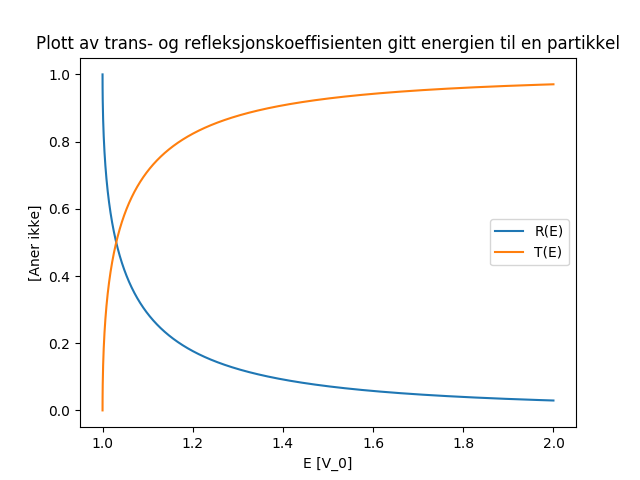
\includegraphics[width=12.6cm,height=9cm]{Figur_05.png}
\lstinputlisting{Oblig8_1c.py}
\end{document}